\chapter{Preintegrated sensors}
\minitoc

% \section{Motion integration}
% First, as a motivational example, we will look at a simple 2D integration motion integration problem. 
% Let's define the state of our robot as the pose $\T{w}{b} \in \SE (2) or \SE(3)$. 
% Let's assume we have a source of odometry, coming from wheel encoders for instance, providing velocity measurements in the base frame 
% $\bfz_k = [\vel{b}{}, \angvel{b}{}]_k$. Now, to update our current estimate of the state, we just have integrate during \dt (one step) 
% using the matrix exponential, as seen in ..., to create a instantaneous relative transformation $\delta_k$ and then compose it with our previous step:

% \begin{equation}
%     \begin{split}
%         &\delta_k = \Exp(\bfz_k * \dt) 
%         \\
%         &\T{}{}^k = \T{}{}^k \delta_k
%     \end{split}
% \end{equation}

% Now, assume that we a set of such measurements between 2 \KFs $i$j and $j$ $\mathcal{Z_{im}} = [\tilde\bfz_k]_{i..j}$. 
% For high frequency sensors, integration is costly. We want to do it once and for all.
% We need to integrate the measurements the two \KFs timestamp in order to obtain a single measurement and derive a factor out of it.
% In this example, this is simply done by composing the $\delta_k$ recursively one at a time.

% \begin{equation}
%     \T{}{j} = \T{}{i} \prod_{k=i}{j}\delta_k = \T{}{i} \tilde\Delta_{im}
% \end{equation}

% Then a residual can be created using the $\Log$ operator:

% \begin{equation}
%     \bfr(\T{}{i}, \T{}{j}) = \Log(\T{}{i}^{-1}\T{}{j} \tilde\Delta_{im})
% \end{equation}

% However, in some cases, those velocity measurements are biased, due to a modeling error, for instance a wrong wheel radius. 
% To obtain meaningful estimations, we need to model this bias and include it in our estimation problem. If we consider a simple additive bias in our example
% $\tilde\bfz_k = \bfz_k + \bfb$, we see that the resulting $\tilde\Delta(\bfb)$ measurements depend on $\bfb$ in a non trivial way. Therefore,
% each time a numerical comes up with a new estimate for $\bfb$, to compute the exact $\tilde\Delta(\bfb)$, the integration of $\mathcal{Z_{im}}$ 
% needs to be recomputed which is computationally costly. As we will see in the next section, this is solved by linearizing $\tilde\Delta(\bfb)$ with respect to $\bfb$ around
% the bias $\ol\bfb$ that was estimated at the time of the integration. 

% On the other end, for other kind of sensors (such as IMUs), it is harder to make the distinction between a delta quantity only depending on raw measurement (and an occasional estimated bias).
% We have therefore to find special coordinate systems in which to integrate measurements in order to obtain an efficient algorithm. To obtain a factor, we also need to consider integrate 
% noise odometry noise at each step to obtain the total covariance of the integrated motion.

% These foundational ideas introduced in \cite{lupton-09}



  
\section{A motivational example: IMU integration for graph optimization}
In this section we will introduce the IMU measurement model and explain why integrating these measurements in the world frame does not immediately
lead to a viable factor. We will then explain the observations that lead to the development of the IMU pre-integration algorithm by Lupton \cite{lupton-09}.

Let's consider the estimation of a robot base pose and velocity in the world frame. We will neglect effects due the rotation of the earth by assuming 
that our world frame (which is fixed wrt. the ground) is an inertial frame, which
is a common simplification in robotics scenarios \cite{forster2017-TRO}. Without loss of generality, we assume that the IMU frame is identical to the base frame 
in the following developments. Among available sensors, the IMU measurements are known to be noisy, biased, and affected by the gravity.

\begin{equation}
    \begin{split}
    \angvelm{}{} &= \angvel{B}{WB} + \bias_{\angvel{}{}} + \noise_{\angvel{}{}} 
    \\
    \accm{}{}    &= \Rot{B}{W} \grav + \acc{B}{WB} + \bias_{\acc{}{}} + \noise_{\acc{}{}} 
    \end{split}
    \label{eq:imu_meas_model}
\end{equation}
    
Other sensors can help estimate IMU biases so we include the biases in the estimator state.

\begin{equation}
    \bfx = [\posi{W}{WB}, \vel{W}{WB}, \Rot{W}{B}, \bias_{\bfa}, \bias_{\angvel{}{}}]
    \triangleq 
    [\bfp, \bfv, \Rot{}{}, \bias_{\bfa}, \bias_{\angvel{}{}}] 
\end{equation}

Once the IMU has been started, these biases slowly change over time, depending on the quality of the IMU used. This change is almost always modeled 
as a random walk which is close to the observed behavior for rather short periods of time \cite{hussen2015low}.
A dynamical model based on strapdown integration of IMU measurements can then be derived.
%
\begin{equation}
    \begin{split}
    \dot{\posi{}{}} = \vel{}{}  ~~~~~~~
    \dot{\vel{}{}} = \acc{W}{WB} ~~~~~~~
    \dot{\Rot{}{}} = \Rot{}{} [\angvel{B}{WB}]_{\times} ~~~~~~~
    \dot{\bias}_{\bfa} = \noise_{\bfa}  ~~~~~~~
    \dot{\bias}_{\angvel{}{}} = \noise_{\angvel{}{}} ~~~~~~~
    \end{split}
    \label{eq:imu_dyn_conti}
\end{equation}
%
Introducing the measurement equations \eqRef{eq:imu_meas_model} in continuous dynamics \eqRef{eq:imu_dyn_conti} and using a zero order hold
explicit Euler integration scheme during $\dt$ results in the discrete dynamics:

\begin{equation}
    \begin{split}
    \Rot{}{}^{k+1}  &= \Rot{}{}^{k}\Exp((\angvelm{}{}^k - \bias_{\angvel{}{}}^k - \noise_{\angvel{}{}}^k)\dt)
    \\
    \vel{}{}^{k+1}  &= \vel{}{}^{k} + \grav \dt + \Rot{}{}^{k}(\accm{}{}^k - \bias_{\acc{}{}}^k - \noise_{\acc{}{}}^k)\dt
    \\
    \posi{}{}^{k+1} &= \posi{}{}^{k} + \vel{}{}^{k}\dt + \frac{1}{2}\grav \dt^2 
    + \frac{1}{2}\Rot{}{}^{k}(\accm{}{}^k - \bias_{\acc{}{}}^k - \noise_{\acc{}{}}^k)\dt^2
    \end{split}
    \label{eq:imu_dyn_disc}
\end{equation}
    
Now, these equations relate variables variables between two state variables sampled at IMU frequency. To include these measurements in our smoothing estimator,
one solution would be to introduce new variables at the rate of the IMU. However, the size of the problem would grow very quickly. A better option
is to integrate IMU measurements during extended periods of time. If we simply integrate the sequence of IMU measurements $\mathcal{Z}_{im}$ between timestamps 
$t_i$ and $t_m$ by unfurling \eqRef{eq:imu_dyn_disc}, we obtain:
%
\begin{equation}
    \begin{split}
    \Rot{}{}^{m}  &= \Rot{}{}^{i} \prod_{k=i}^{m} \Exp((\angvelm{}{}^k - \bias_{\angvel{}{}}^k - \noise_{\angvel{}{}}^k)\dt) \\
    \vel{}{}^{m}  &= \vel{}{}^{i} + \sum_{k=i}^{m} \Big[\grav \dt + \Rot{}{}^{k}(\accm{}{}^k - \bias_{\acc{}{}}^k - \noise_{\acc{}{}}^k)\dt \Big]  \\
    \posi{}{}^{m} &= \posi{}{}^{i} + \sum_{k=i}^{m} \Big[\vel{}{}^{k}\dt + \frac{1}{2}\grav \dt^2 
    + \frac{1}{2}\Rot{}{}^{k}(\accm{}{}^k - \bias_{\acc{}{}}^k - \noise_{\acc{}{}}^k)\dt^2 \Big]
    \end{split}
    \label{eq:IMUIntij}
\end{equation}
%
Assuming IMU biases stay constant during $\Dt^{im}$, 
\begin{equation*}
    \bias^i \triangleq [\bias_{\acc{}{}}^i, \bias_{\angvel{}{}}^i] \approx [\bias_{\acc{}{}}^k, \bias_{\angvel{}{}}^k]  ~~~ \forall k \in [i..m]
\end{equation*}
% \begin{equation*}
%     \bias_i \triangleq [\bias_{\acc{}{}i}, \bias_{\angvel{}{}i}] \approx [\bias_{\acc{}{}k}, \bias_{\angvel{}{}k}]  ~~~ \forall k \in [i..j]
% \end{equation*}
% \begin{equation*}
%     \bias_i \triangleq [\bias_{\acc{}{},i}, \bias_{\angvel{}{},i}] \approx [\bias_{\acc{}{},k}, \bias_{\angvel{}{},k}]  ~~~ \forall k \in [i..j]
% \end{equation*}
%
we could then directly derive a factor with an error between the expected delta $\hat\bfDelta_{im}$ and the measured delta $\bfDelta_{im}$ defined as:
% $e(\bfx^i, \bfx^j) = \bfDelta_{\bfx}(\bfx^i, \bfx^j)  \ominus  \bfDelta_{\mathcal{Z}_{im}}(\bias^i, \bfx^i)$
%   where 
%
\begin{align}
    \hat\bfDelta_{im}(\bfx^i, \bfx^m) = 
    \begin{bmatrix}
    \Rot{}{}^{i,T} \Rot{}{}^{m}  \\
    \vel{}{}^{m}  - \vel{}{}^{i}  \\
    \posi{}{}^{m} - \posi{}{}^{i}
    \end{bmatrix}
\end{align}
%
and 
%
\begin{align}
    \bfDelta^{im}(\bias^i, \bfx_i) = 
    \begin{bmatrix}
    \prod_{k=i}^{m} \Exp((\angvelm{}{}^k - \bias_{\angvel{}{}}^i)\dt)  \\
    \sum_{k=i}^{m} \Big[\grav \dt + \Rot{}{}^{k}(\accm{}{}^k - \bias_{\acc{}{}}^i - \noise_{\acc{}{}}^k)\dt \Big]  \\
    \sum_{k=i}^{m} \Big[\vel{}{}^{k}\dt + \frac{1}{2}\grav \dt^2 
    + \frac{1}{2}\Rot{}{}^{k}(\accm{}{}^k - \bias_{\acc{}{}}^i)\dt^2 \Big]
    \end{bmatrix}
\end{align}
%
Both quantities are recomputed at each evaluation of the residual by the nonlinear solver. $\bfDelta_{\bfx}(\bfx_i, \bfx_m)$ is fairly quick to compute.
However $\bfDelta_{\mathcal{Z}_{im}}(\bias^i, \bfx_i)$ formulation requires to reintegrate the whole buffer of measurements which
is highly inefficient. This is due to the dependency on velocity, orientation and biases at timestamp $i$. However the terms of equation \eqRef{eq:IMUIntij} can 
be rearranged (proof in the annex -> TODO) to give:
%
% WITH NOISE
% \begin{equation}
%     \begin{split}
%     \bfDelta \Rot{}{im} &\triangleq  \Rot{}{}^{i,T} \Rot{}{}^{m} =  \prod_{k=i}^{m} \Exp((\angvelm{}{}^k - \bias_{\angvel{}{}^k} - \noise_{\angvel{}{}^k})\dt) \\
%     \bfDelta \vel{}{im} &\triangleq \Rot{}{}^{i,T} (\vel{}{j} - \vel{}{i} - g \Dt^{im}) 
%     = \prod_{k=i}^{m} \bfDelta \Rot{}{ik} \Exp((\accm{}{}^k - \bias_{\acc{}{}}^k - \noise_{\acc{}{}}^k)\dt)  \\
%     \bfDelta \posi{}{im} &\triangleq \Rot{}{}^{i,T}(\posi{}{}^j - \posi{}{}^i - \vel{}{}^i \Dt^{im} - \frac{1}{2} \grav \Dt^{im}^2) 
%     = \sum_{k=i}^{m} \Big[\bfDelta \vel{}{ik}\dt +  \frac{1}{2} \bfDelta \Rot{}{ik} (\accm{}{}^k - \bias_{\acc{}{}}^k - \noise_{\acc{}{}}^k)\dt^2 \Big]
%     \end{split}
%     \label{eq:IMUPreintij}
% \end{equation}
%
\begin{equation}
    \begin{split}
    \DR^{im} &\triangleq  \Rot{}{}^{i,T} \Rot{}{}^{m} =  \prod_{k=i}^{m} \Exp((\angvelm{}{}^k - \bias_{\angvel{}{}}^i)\dt) \\
    \Dv^{im} &\triangleq \Rot{}{}^{i,T} (\vel{}{m} - \vel{}{i} - \grav \Dt^{im}) 
    = \prod_{k=i}^{m} \DR^{ik} \Exp((\accm{}{}^k - \bias_{\acc{}{}}^i)\dt)  \\
    \Dp^{im} &\triangleq \Rot{}{}^{i,T}(\posi{}{}^m - \posi{}{}^i - \vel{}{}^i \Dt^{im} - \frac{1}{2} \grav \Dt^{im,2}) 
    = \sum_{k=i}^{m} \Big[\Dv^{ik}\dt +  \frac{1}{2} \DR^{ik} (\accm{}{}^k - \bias_{\acc{}{}}^i)\dt^2 \Big]
    \end{split}
    \label{eq:IMUPreintij}
\end{equation}
%
where we define $\DR^{ik} \triangleq \Rot{}{i,T} \Rot{}{}^k$.
We then overwrites our delta notations as $\bfDelta_{\bfx,im}(\bfx_i, \bfx_m) = \bfDelta_{\mathcal{Z}_{im}}(\bias^i)$
which lifts the dependency of the right hand term on the initial state $\bfx_i$. However the bias terms in \eqRef{eq:IMUPreintij} still enforce the repeated 
reintegration of the measurements buffer. Instead, the right hand side can be integrated once using biases estimates at the time where we begin to integrate them that
we note $\biasbar_i$. Then, we can approximate changes due to the newly estimated bias $\bias_i$ using a first order approximation.
% $\bfDelta_{\mathcal{Z}_{im}}(\bias^i) = \bar{\bfDelta}_{\mathcal{Z}_{im}} \oplus (\bfJ^{\bfDelta_{\mathcal{Z}_{im}}}_{\bias_i} (\bias^i - \biasbar^i))$.

These two observations were first made by Lupton \cite{lupton-09}, whose formulation relied on Euler angles, and were later formalized on \SO(3) using Lie theory
by Forster \cite{forster2017-TRO}. The above equations are not directly useful for the implementation of pre-integration. We need first to derive a recursive formulation 
of the problem. IMU noise propagation also needs to be described in order to obtain covariances associated to the factor error. In the next section, we will take 
a step back and derive a pre-integration generalized to other proprioceptive sensors.



\section{Generalized pre-integration}
\label{sec:general-preint}


Pre-integration refers to the integration of high rate proprioceptive sensory data in an efficient way in the context of factor graphs. 
It was initially developed to deal with IMU measurements \cite{lupton-09, forster2017-TRO}. 
As we have seen, if a standard integration is conducted naively to derive a factor measurement between two KFs, 
then the IMU data needs to be reintegrated at each solver iteration because the integral depends on the states we are to estimate. 
The IMU pre-integration theory solves this issue and can be generalized to any proprioceptive sensor as shown in \cite{atchuthan-18-thesis,deray-19-selfcalib,fourmy2021contact}. 
Delta quantities $\bfDelta_{im}$  are defined between KFs $i$ and $m$ so that $\bfx_m=\bfx_i\boxplus\bfDelta_{im}$. A suitable composition $\boxplus$ is chosen so that $\bfDelta_{im}$ 
does not depend on the initial states $\bfx_i$. 
Dependence on other small-varying parameters $\bfb$ such as sensor bias is linearized as $\bfDelta_{im}(\bfb)=\bfDelta_{im}(\ol\bfb)\op\bfJ^\bfDelta_\bfb(\bfb-\ol\bfb)$.
Then we can pre-integrate $\ol\bfDelta_{im}\te\bfDelta_{im}(\ol\bfb)$ once during data gathering, and use it to define residuals that are later evaluated many times by the optimizer.
This was the main contribution of paper my paper \cite{fourmy2021contact}.

\subsection{Delta pre-integration}

\begin{figure}[tb]
    \centering
    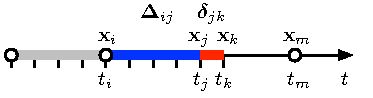
\includegraphics[width=0.6\textwidth]{figures/delta_time}
    \caption{
    The pre-integrated delta $\bfDelta_{ij}$ contains all motion from the last KF at time $i$, up to time $j$. 
    The current delta $\bfdelta_k$ contains the motion from times $j$ to $k$, computed from the last IMU measurement at time $k$.}
    \label{fig:delta_time}
\end{figure}

We perform pre-integration incrementally as follows. 
First, $\ol\bfDelta_{ii}$ is initialized to the null motion. 
Its covariance $\bfSigma_\Delta^{ii}$ and the Jacobian $\mjac{\bm\delta_i}{\bfb_i}$ are set to zero. 
At each reception of sensor data $\tilde\bfz_k$ at $t_k$, we integrate during $\dt$ to obtain the delta corresponding to a single data sample
%
\begin{align}
\bm\delta_k = f(\tilde\bfz_k, \ol\bfb_i, \dt)~, 
\label{eq:data2delta}
\end{align}

using the bias $\ol\bfb_i$ available in KF $i$. 
This single delta is integrated onto the delta pre-integrated so far using the delta composition law

\begin{align}
\ol\bfDelta_{ik} = \ol\bfDelta_{ij} \circ \bm\delta_k~. 
\label{eq:deltaPlusDelta}
\end{align}

which is represented in figure \figRef{fig:delta_time}.
%with Jacobians $\mjac{\ol\bfDelta_{ik}}{\ol\bfDelta_{ij}}$ and $\mjac{\ol\bfDelta_{ik}}{\bm\delta_k}$. 
The Jacobian of the pre-integrated delta with respect to biases, as well as the delta covariance, are also pre-integrated

\begin{align}
    \mjac{\bfDelta_{ik}}{\bfb_i} &= \mjac{\bfDelta_{ik}}{\bfDelta_{ij}}\mjac{\bfDelta_{ij}}{\bfb_i} 
+ \mjac{\bfDelta_{ik}}{\bm\delta_k}\mjac{\bm\delta_k}{\bfb_i} \\
    \bfSigma_\Delta^{ik} &= \mjac{\bfDelta_{ik}}{\bfDelta_{ij}}\bfSigma_\Delta^{ij}\mjac{\bfDelta_{ik}}{\bfDelta_{ij}}\tr 
+ \mjac{\bfDelta_{ik}}{\bm\delta_k}\mjac{\bm\delta_k}{\bfz_k}\bfSigma_\bfz\mjac{\bm\delta_k}{\bfz_k}\tr\mjac{\bfDelta_{ik}}{\bm\delta_k}\tr
\end{align}

where $\mjac{\bm\delta_k}{\bfb_i}$, $\mjac{\bm\delta_k}{\bfz_k}$, $\mjac{\bfDelta_{ik}}{\bfDelta_{ij}}$ and $\mjac{\bfDelta_{ik}}{\bm\delta_k}$ 
are the Jacobians $\mjac{y}{x}=\partial y/\partial x$ of (\eqRef{eq:data2delta},\eqRef{eq:deltaPlusDelta}), computed according to Lie theory \cite{sola2018micro}.


\subsection{Residual definition}
\label{sec:preint_residual}

The pre-integrated $\ol\bfDelta_{im}$ is used at the end of the pre-integration to define the residual

\begin{align}
    \bfr_{im} = (\ol\bfDelta_{im} \oplus \mjac{\bfDelta_{im}}{\bfb_i}(\bfb_i-\ol\bfb_i) ) \ominus \hat\bfDelta_{im}
    \label{eq:preint_residual}
\end{align}

where $\bfb_i$ is the current bias value,  $\hat\bfDelta_{im}=\bfx^m\boxminus\bfx^i$ is the expected delta between KFs, and $\{\op,\om\}$ are the composite
 plus and minus operators described in \cite{sola2018micro}. 
That is, $\{\op,\om\}$ are $\{+,-\}$ for vectors, and for rotations we have $\bfR\op\bm\theta\te\bfR\Exp(\bm\theta)$ and $\bfR_2\om\bfR_1\te\Log(\bfR_1\tr\bfR_2)$. 
The residual clearly depends on the KF states $\bfx^i,\bfx^m$ and the bias $\bfb_i$. It has an associated covariance  $\bfSigma_\Delta^{im}$.



\subsection{IMU pre-integration}

The states involved in this integration are the base states $\bfx_b = [\posi{}{}, \bfv, \Rot{}{}]$ with deltas $\bfDelta=[\Dp,\Dv,\DR]$. 
The IMU produces biased and noisy measurements $\tilde\bfz = [\tilde\bfa, \tilde{\bfomega}]$ of the base proper acceleration and angular velocity, 
with bias $\bfb = [\bias_{a}, \bias_{\omega}]$ and noise $\noise = [\noise_{a}, \noise_{\omega}]$. 

The pre-integration method in  \cite{forster2017-TRO} can be put in the formalism above by realizing that defining $\bm\delta=f(\tilde\bfz,\bfb,\dt)$ in \eqRef{eq:data2delta} as

\begin{align}
    \bm\delta^k = \begin{bmatrix}
    \delta\bfp\\\delta\bfv\\\delta\bfR
    \end{bmatrix}^k =
    \begin{bmatrix}
    \tfrac12(\tilde\bfa-\bfb_a-\noise_a)\dt^2 \\
    (\tilde\bfa-\bfb_a-\noise_a)\dt \\
    \Exp((\tilde{\bfomega}-\bfb_\omega-\noise_\omega)\dt)
    \end{bmatrix}^k
\end{align}

and the composition law $\bfDelta^{ik}=\bfDelta^{ij}\circ\bm\delta^k$ in \eqRef{eq:deltaPlusDelta} as

\begin{align} \label{eq:composition_delta}
    \begin{split}
    \Dp^{ik} 
    &= \Dp^{ij} + \Dv^{ij}\dt + \DR^{ij}\dpp^{k} \\
    \Dv_{ik} 
    &= \Dv^{ij} + \DR^{ij}\dv^{k} \\
    \DR^{ik} 
    &= \DR^{ij}\dR^{k} 
    \end{split}
\end{align}

then $\bfx_k=\bfx_i\boxplus\bfDelta_{ik}$ is \cite[eq.~32]{forster2017-TRO} and $\bfDelta_{ik}=\bfx_k\boxminus\bfx_i$ is \cite[eq.~33]{forster2017-TRO}. 
Full details can be found in \cite[Section 3.4]{atchuthan-18-thesis}.



%
%
%
%
\section{IMU pre-integration on Lie groups}
In \cite{fourmy2019absolute}, we showed that an alternative formulation of IMU preintegration on Lie groups was possible.
We introduce a new matrix Lie group representation of
the IMU deltas. The complete IMU pre-integration theory,
including the computation of the residual, is based on this
new Lie structure. The theoretical material for the Lie
development in this section can be found in the report \cite{sola2018micro}.
% For some developments and formulae related to the particular
% IMU case, please refer to the appendix.

\subsection{Lie Group formulation}

We propose a matrix form of the Lie group of IMU deltas as,
%
\begin{align}\label{equ:delta_Lie}
\D &= 
\begin{bmatrix}
\DR & \Dv & \Dp \\
\bf0 & 1 & \Dt \\
\bf0 & 0 & 1
\end{bmatrix} \in \cD \subset \bbR^{5\times 5}
~.
\end{align}

Group identity, inverse and composition stem from regular matrix identity, inverse (with $\DR\inv=\DR\tr$) and product,

\begin{align}
\D_\cE&=\begin{bmatrix}
\bfI & \bf0 & \bf0 \\
\bf0 & 1 & 0 \\
\bf0 & 0 & 1 
\end{bmatrix} = \bfI_{5\times5}
\label{equ:identity}
\\
\D\inv &= \begin{bmatrix}
\DR\tr & -\DR\tr\Dv & -\DR\tr(\Dp-\Dv\Dt) \\
\bf0 & 1 & -\Dt \\
\bf0 & 0 & 1
\end{bmatrix} 
\label{equ:inverse}
\\
\D\cdot\bm\delta 
&= 
\begin{bmatrix}
\DR\dR & \Dv + \DR\dv & \Dp+\Dv\dt + \DR\dpp \\
\bf0 & 1 & \Dt+\dt \\
\bf0 & 0 & 1
\end{bmatrix}
~.
\label{equ:composition}
\end{align}
%
% Comparing against \eqsRef{equ:composite_identity}{equ:composite_composition} we observe that this matrix Lie group is exactly equivalent to the classical IMU deltas above.



\subsubsection{Lie algebra \texorpdfstring{$\mathfrak{d}$}{d} and exponential map}

The Lie algebra elements $\bftau\hhat$ and their isomorphic Cartesian $\bftau$ have the forms
%
\begin{align}\label{equ:lie_algebra}
    \bftau\hhat &= \begin{bmatrix}
    \hatx{\bth} & \bfrho & \bfupsilon \\
    \bf0 & 0 & \Dt \\
    \bf0 & 0 & 0
    \end{bmatrix} \in \mathfrak{d}
    ,&
    \bftau &= \begin{bmatrix}
    \bfrho \\ \bfupsilon \\ \bth \\ \Dt
    \end{bmatrix}
    \te \begin{bmatrix}
    \bfv\Dt \\ \bfa\Dt \\ \bw\Dt \\ \Dt
    \end{bmatrix} 
    \in \bbR^{10}
    ,
\end{align}
%
with $\bfv\te\dot\Dp$, $\bfa\te\dot\Dv$ and $\hatx{\bw}\te\DR\tr\dot\DR$.
Operators $\wedge$ and $\vee$ are defined so that $\bftau\hhat=(\bftau)\hhat$ and $\bftau=(\bftau\hhat)\vvee$.

The exponential map transfers tangent elements to the group; the logarithmic map is its inverse,
%
\begin{align}
    \D &= \Exp(\bftau) \te \exp(\bftau\hhat) = \begin{bmatrix}
    \Exp(\bth) & \bfQ\bfupsilon & \bfQ\bfrho+\bfP\bfupsilon\Dt \\
    \bf0 & 1 & \Dt \\
    \bf0 & 0 & 1
    \end{bmatrix} %\in\cD 
    \label{equ:exp}
    \\
    \bftau &= \Log(\D) \te \log(\D)\vvee = \begin{bmatrix}
    \bfQ\inv(\Dp-\bfP\bfQ\inv\Dv\Dt) \\
    \bfQ\inv\Dv \\
    \Log(\DR) \\
    \Dt 
    \end{bmatrix} %\in \bbR^{10}
    \label{equ:log}
\end{align}
%
where $\Log()$ is obtained by identifying terms in \eqRef{equ:delta_Lie} and \eqRef{equ:exp}.
Matrices $\bfP$ and $\bfQ$ are provided in the appendix.


\subsubsection{Jacobians, uncertainty}
\label{sec:uncertainty}

For general functions $f:\cM\to\cN;y=f(x)$, we propagate uncertainty normally via the Jacobians $\mjac{y}{x}\te\dpar{y}{x}$, \ie, $\bfSigma_y=\mjac{y}{x}\,\bfSigma_x\,\mjac{y}{x}\tr$. 
These Jacobians map the tangent spaces of the mannifolds $\cM,\cN$ at $x$ and $y$, and in case of vector spaces they resort to the classical Jacobian.
They also satisfy the chain rule, which we use extensively in our developments.
We provide ample reference and justification of this approach in the technical report \cite{sola2018micro}.

A comment is however necessary for the present IMU case.
It relates to the uncertainty of the last component of the tangent space \eqRef{equ:lie_algebra}, which is the time $\Dt$. This component has no uncertainty by definition. 
Having it in the covariances would imply singularity and result in the risk of a number of well-known numerical issues. 
We therefore systematically marginalize this time component out of the covariances, simply by removing the last row and column. 





\subsubsection{Delta Lie group IMU factor residual}
Computation of the residual in the case of the Lie Delta group formulation follows the steps defined in \secRef{sec:general-preint}.
However, since the Delta is directly defined as a Lie group, the formulation is actually simplified because  ... 
Use the pre-integrated Jacobian $\mjac{\D_{im}}{\bfb}$ to correct the pre-integrated delta $\ol\D_{im}$ to account for the new bias estimate $\bfb_i\neq\ol\bfb_i$,

\begin{align}
    \D_{im}(\bfb_i) &= \ol\D_{im}\cdot\Exp(\mjac{\D_{im}}{\bfb}(\bfb_i-\ol\bfb_i)) 
    ~.
\end{align}

Use [Forster delta def] \eqRef{equ:delta} as $\boxminus$ to compute the expected delta from  $\bfx_i$ to $\bfx_m$,

\begin{align}
    \widehat\D_{im}(\bfx_i,\bfx_m) &= \bfx_m \boxminus \bfx_i 
    ~.
\end{align}
Compute the residual in the  tangent of $\cD$ at $\D_{im}$,

\begin{align}
    \bfr^\Delta_{im}(\bfx_i,\bfx_m,\bfb_i) &= \Log(\D_{im}(\bfb_i)\inv \cdot \widehat\D_{im}(\bfx_i,\bfx_m)) \in \bbR^9
~,
\end{align}

and drop the $\Dt$ part from the residual after the $\Log()$ ---see comment in \secRef{sec:uncertainty}.
In this last equation, the composite minus operator $\oplus$ is simply the traditional Lie group "minus" operator defined in [cite sola eq ...] applied
between the corrected preintegration delta and the expected delta.



\subsection{IMU Lie group versus Forster's method}

Mathematically, and disregarding methodology, the main difference between our method and Forster's \cite{forster2017-TRO} is to be found in the exponential map. 
To see it, let us consider small rotation increments $\bth=\bw\dt$ captured at each single IMU sample. 
In such cases, the matrices $\bfP,\bfQ$ appearing in the exponential map \eqRef{equ:exp} and detailed in \eqRef{equ:RQP} can be approximated by $\bfP\approx\tfrac12\bfI$ and $\bfQ\approx\bfI$.
The exponential becomes,
%
\begin{align}
    \Exp\left(\begin{bmatrix}
    \bf0 \\ \bfa \\ \bw \\ 1
    \end{bmatrix}\dt\right) \approx \begin{bmatrix}
    \Exp(\bw\dt) & \bfa\dt & \tfrac12\bfa\dt^2 \\
    \bf0 & 1 & \dt \\
    \bf0 & 0 & 1
    \end{bmatrix}
~,
\end{align}
%
where we find the terms $\bfa\dt$ and $\tfrac12\bfa\dt^2$, which should sound familiar from Forster's method. 
In effect, with this approximation, if we now compact all the steps \eqsRef{equ:pre_calibration}{equ:pre_composition} of our integration into a cumulative expression,
%
\begin{align}
    \D_{ik} = \prod_{j=i+1}^k \Exp\left(\begin{bmatrix}
    \bf0 \\ (\bfa_j-\bfa_{bi}) \\ (\bw_j-\bw_{bi}) \\ 1
    \end{bmatrix}\dt\right)
~,
\end{align}
%
it is possible (although tedious) to show that both Forster's and our method are exactly equivalent when $\bw\dt\to0$.
% , which is usually a valid hypothesis.
% These differences should not constitute an argument against Forster, since in practice we typically have extremely small steps $\bw\dt$ and the approximation holds very well.









\section{External force pre-integration}
In this section we apply the generalized pre-integration algorithm to the problem of using measured external
forces applied on a legged robot in a smoothing estimator. We propose to integrate the underactuated that we first recall. Then 
we derive the specificities of the pre-integration of external forces of a poly-articulated system. This is the main theoretical contribution
of our paper \cite{fourmy2021contact}.


\subsection{Centroidal kinematics}
The robot dynamics is described by the well-known:
\begin{equation}\label{eq:wbdyn}
  \bfM(\q) \vq + h(\q,\vq) = \bm\tau_q + \sum_l \bfJ_l\tr \bff_l
\end{equation}
where $\q,\vq,\dvq,\bm\tau_q$ are the position, velocity, acceleration and torques of the robot in configuration space,
$\bff_l$ are the contact forces (written as 3D forces in this paper),
$\bfM$ is the generalized inertia matrix, $h$ the sum of gravity, Coriolis and centrifugal forces, and $\bfJ_l$ the jacobians of the contact points.
Because of the underactuated nature of legged robots, the configuration is often separated into $\q=(\posi{W}{B},\Rot{W}{B},\qa)$ where $\posi{W}{B}$ 
is the position in world frame of the robot base (typically, the torso or in our case the IMU), $\Rot{W}{B}$ the rotation of the base body with respect 
to the world and $\qa$ are the joint configuration of the actuated joints. 
%We will subsequently use the notation $\prescript{X}{}{[\cdot]}_Y$ to denote vectorial quantities of frame $Y$ expressed in frame $X$. A tilde $\Tilde{[\cdot]}$ denotes a noisy measurement.

While~\eqRef{eq:wbdyn} represents the whole dynamics, a subpart of it is of particular importance for legged robots.
The centroidal dynamics is written by the two equations:
%
\begin{equation}
    m \ddot{\bfc} = m \bfg + \sum_l \bff_l \quad , \quad
\dAM = \sum_l (\posi{}{l} - \COM) \times \bff_l
\label{eq:NewtonEuler}
\end{equation}
%
where $\COM,\AM$ are the position of the Center of Mass (CoM) and Angular Momentum (AM) around the CoM (both expressed in world frame), $m$ is the robot total mass, 
and the $\posi{}{l}$ are the positions of the contact points in world frame. The centroidal dynamics is an exact part of \eqRef{eq:wbdyn} and more deeply reveals 
the underactuation: the robot can move only if applying the proper forces to the environment, as the joint torques alone cannot lead to any modification 
of CoM or AM.


The classical approach in estimation of legged robot state is to first estimate the base state, and then to reconstruct the centroidal state $(\bfc,\dot{\bfc},\AM)$ using the joint position and velocity measurements, and the robot model.
This assumes that there is no direct measurement of the centroidal state.
Consequently, we are not be able to recover the exact centroidal state if there is any bias in the robot model.

Yet, we can see from the centroidal dynamics that the force measurements are connected to the variation of the centroidal state.
As observed in~\cite{carpentier2016center}, a proper fusion of the force measurements with an estimation of the state of the base makes the centroidal state observable.


\subsection{Force pre-integration factor}

The Newton-Euler equations \eqRef{eq:NewtonEuler} relate the evolution of the CoM and AM due to gravity, external forces and torques. 
In the case of a legged robot with punctual contact feet, only forces $\forcem{}{L}$ are applied at each limb contact $L$, with no torque. 
We assume that at each  limb contact we have access to noisy local force measurements $\forcem{}{L} = \force{L}{L} + \noise_f$. 
To transform them into the body frame $b$, we compute $\Rotm{}{L} \triangleq \Rot{B}{L}(\qa)  \in SO(3)$ and $\posim{}{L} \triangleq \posi{B}{L}(\qa) \in \Reals^3 $ from the joint configuration $\qa  \in \Reals^{12}$. 
The lever arm $(\posi{}{L}-\bias_c)$ in \eqRef{eq:NewtonEuler} uses a measurement of the CoM position in base frame $ \posi{B}{C}(\qa) \in \Reals^3$. 
This measure is biased due to inaccuracies in the robot model and therefore we add a bias variable to be estimated, $\bias_c \in \Reals^3$ so that $\posim{}{C} = \posi{B}{C}(\qa) + \bias_c + \noise_c$.
Assuming constant forces during each interval $\dt$ 
the integration of \eqRef{eq:NewtonEuler} yields the discrete dynamic model for the centroidal states:
%
\begin{equation}
\begin{split}
\COM^{k} &= \COM^{k-1} + \COMd^{k-1} \dt+\frac{1}{2} \bfg \dt^2 + \frac{1}{2m} \Rot{}{}^{k-1} \sum_L \Rotm{}{L}^k (\forcem{}{L}^k - \noise_{f}) \dt^2
\\
\COMd^{k}&= \COMd^{k-1} + \bfg \dt + \frac{1}{m} \Rot{}{}^k \sum_L\Rotm{}{L}^k (\forcem{}{L}^k - \noise_{f}) \dt 
\\
\AM^{k} &= \AM^{k-1} +\Rot{}{}^k \sum_L (\posim{}{L}^k  - \posim{}{C}^k +  \bias_{c}^k + \noise_{c}) \times \Rotm{}{L}^k(\forcem{}{L}^k - \noise_{f}) \dt
\end{split}
\label{eq:COMDiscrete}
\end{equation}
%
Analogously to the IMU case, it is possible to pre-integrate force measurements to derive a factor on the states 
$\bfx_c=[\COM, \COMd, \AM, \Rot{}{}]$ using deltas $\D_c=[\D\COM, \D\COMd, \D\AM, \DR]$. 
The rotation measured by the gyroscope has to be included too for the pre-integration to work. 
In this case, the bias vector is $\bias = [\bias_c, \bias_{\omega}]$. We define measurements  $\bfz^k$ to be:
%
\begin{equation}
\bfz^k = \left[ \posim{}{C}^k, \angvelm{}{}^k, \left[\forcem{}{L}^k, \posim{}{L}^k, \Rotm{}{L}^k \right]_{L=1..4}\right]
\end{equation}

The following operators are enough to particularize the  method in \secRef{sec:general-preint} to the contact forces case.
Integrating $\bfz_k$ during $\dt$ yields $\bm\delta_k$ in \eqRef{eq:data2delta} as
%
\begin{equation}
\small
    \bm\delta^{k}(\bfz^k, \bfb^i, \dt) =
    \begin{bmatrix}
    \frac{1}{2m} \sum_l \Rotm{}{L}^k \forcem{}{L}^k \dt^2
    \\
    \frac{1}{m} \sum_l \Rotm{}{L}^k \forcem{}{L}^k \dt 
    \\
    (\sum_l \posim{}{L}^k - (\posim{}{C}^k - \bias_c^i) \times (\Rotm{}{L}^k \forcem{}{L}^k ))\dt
    \\
    \Exp((\angvelm{}{}^k - \bias_{\omega}^i)\dt)
    \end{bmatrix}
\normalsize
\end{equation}
%
and the delta composition law in \eqRef{eq:deltaPlusDelta} as
%
\begin{equation}
    \D \circ \bm\delta = 
    \begin{bmatrix}
    \D\COM + \D\COMd \dt + \DR  \delta\COM
    \\
    \D\COMd + \DR  \delta \COMd
    \\
    \D\AM + \DR  \delta \AM
    \\
    \DR\dR
    \end{bmatrix}
    ~.
    \label{eq:DeltaDTCompo}
\end{equation}
%
The expected delta $\D^{ik}=\bfx^k\boxminus\bfx^i$ between KFs $i$ and $k$ reads
%
\begin{equation}
\D^{ik} =
\begin{bmatrix}
   \D\COM^{ik} \\ \D\COMd^{ik} \\ \D\AM^{ik} \\ \DR^{ik}
\end{bmatrix}
=
\begin{bmatrix}
	{\Rot{}{}^i}\tr (\COM^k - \COM^i - \COMd^i \Dt^{ik})
	\\
	{\Rot{}{}^i}\tr (\COMd^{k} - \COMd^{i} - \bfg \Dt^{ik})
	\\
	{\Rot{}{}^i}\tr (\AM^{k} - \AM^{i})
	\\
    {\Rot{}{}^i}\tr \Rot{}{}^k
\end{bmatrix}
~.
\end{equation}
%
Finally, the propagation of the state $\bfx_i$ to $\bfx_k$ using $\D_{ik}$, which can be used to retrieve a state at any time $k$ between KFs in the trajectory, is
%
\begin{equation}
	\bfx^k = \bfx^i \boxplus \D^{ik} =
	\begin{bmatrix}
	\COM^i + \COMd^i \Dt^{ik} + \Rot{}{}^i \Delta \COM^{ik} + \frac{1}{2} \bfg \Dt^{ik,2}
	\\
	\COMd^i + \Rot{}{}^i \Delta \COMd^{ik} + \grav \Dt^{ik}
	\\
	\AM^i + \Rot{}{}^i \Delta \AM^{ik}
	\\
	\Rot{}{}^i \DR^{ik}
	\end{bmatrix}
\end{equation}
%
%
%
%


\section{Related works}

\cite{hartley2018legged}
\cite{wisth2020preintegrated}
\cite{lupton-09}
\cite{forster2017-TRO}
GTSAM new IMU preint (?)
\cite{eckenhoff2019closed}
\cite{brossard2021associating}
\cite{luo2021unified} 